%!TEX ROOT=radek-novotny-bp-2017.tex
%%% ML: v teto kapitole obecne chybi zdroje, reference
%%% RN: Doplneny reference, jeste chybi u Grass doplnim
\chapter{Technologie}
\label{3-technologie}
Cílem této kapitoly je v krátkosti popsat technologie, jež byly
použity pro implementaci teoretických poznatků do softwarového
nástroje – zásuvného modulu pro QGIS.
\section[QGIS]{QGIS 
\includegraphics[scale=0.055]{./pictures/qgis.png} 
\footnote{http://www.qgis.org/}}
\label{qgis}
\begin{figure}[H]
    \centering 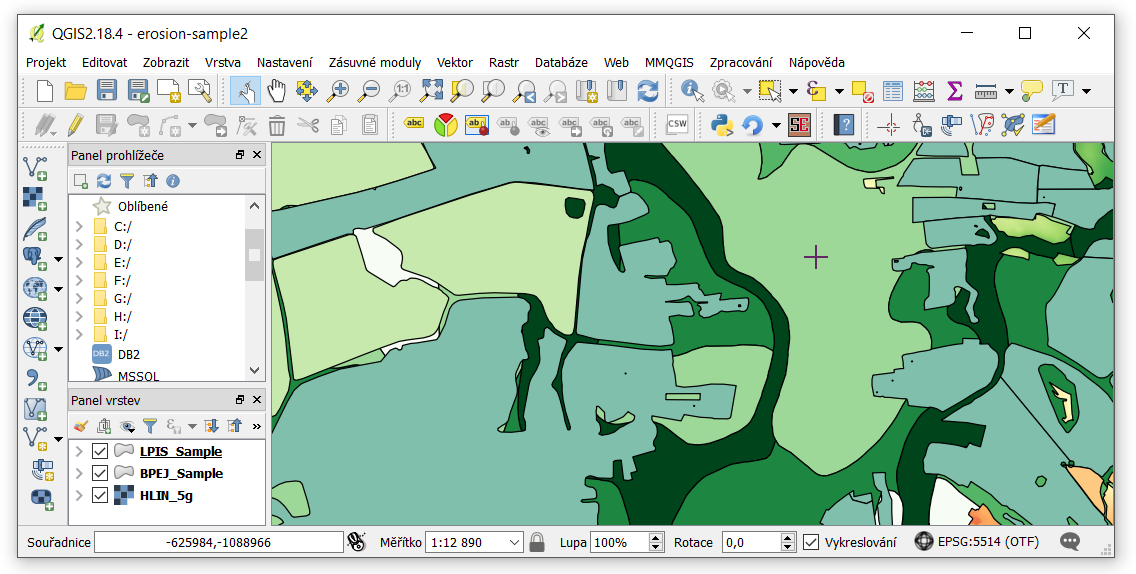
\includegraphics[scale=0.6]{./pictures/qgis_screen.png}
      \caption[Náhled prostředí QGIS 2.18]
      {Náhled prostředí QGIS 2.18, zdroj: autor}
      \label{screen:qgis}
\end{figure}
QGIS, jehož název vychází z původně používaného Quantum GIS, je open
source (licence GNU/GPL) geografický informační systém (GIS) dostupný
z platforem Mac OS X, Linux, Unix, a Microsoft Windows, přičemž od
roku 2014 je vyvíjena i verze pro Android. Samotný vývoj QGIS začal
Gary Sherman v roce 2002, poté byl projekt zařazen do Open Source
Geospatial Foundation (2007) a v roce 2009 vyšla jeho první verze. V
současnosti je aktuální verzí 2.18, jež by měla být poslední v druhé
řadě, přičemž by měla být nahrazena verzí 3.0, která bude postavena na
Python 3 s Qt5 a PyQt5. Od svého vzniku je QGIS udržován a dále
vyvíjen dobrovolníky.

QGIS podporuje většinu funkcí, které jsou od GIS očekávány, ať už se
jedná o podporu mnoha vstupních formátů vektorových i rastrových dat,
výběr a úpravy objektů nebo práci s atributovými tabulkami. Výhodou je
rovněž podpora nástrojů GRASS GIS, pomocí kterých jsou zvládány
složitější výpočetní operace.  Silnou stránkou jsou rovněž zásuvné
moduly (pluginy). Díky rozsáhlé uživatelské komunitě v akademickém,
ale stále častěji i profesním prostředí, a veřejné licenci GNU/GPL,
pod kterou celý QGIS funguje, je vývoj nových zásuvných modulů značně
zjednodušen. V QGIS je pluginů velké množství, čímž se významně
rozšiřují možnosti práce se softwarem. Zásuvný modul pro QGIS je i
výsledkem této práce.\cite{masteringQgis}
\section[GRASS GIS]{GRASS GIS 
\includegraphics[scale=0.12]
{./pictures/grass.png} \footnote{https://grass.osgeo.org/download/logos/}}
\label{grassgis}
\begin{figure}[H]
    \centering 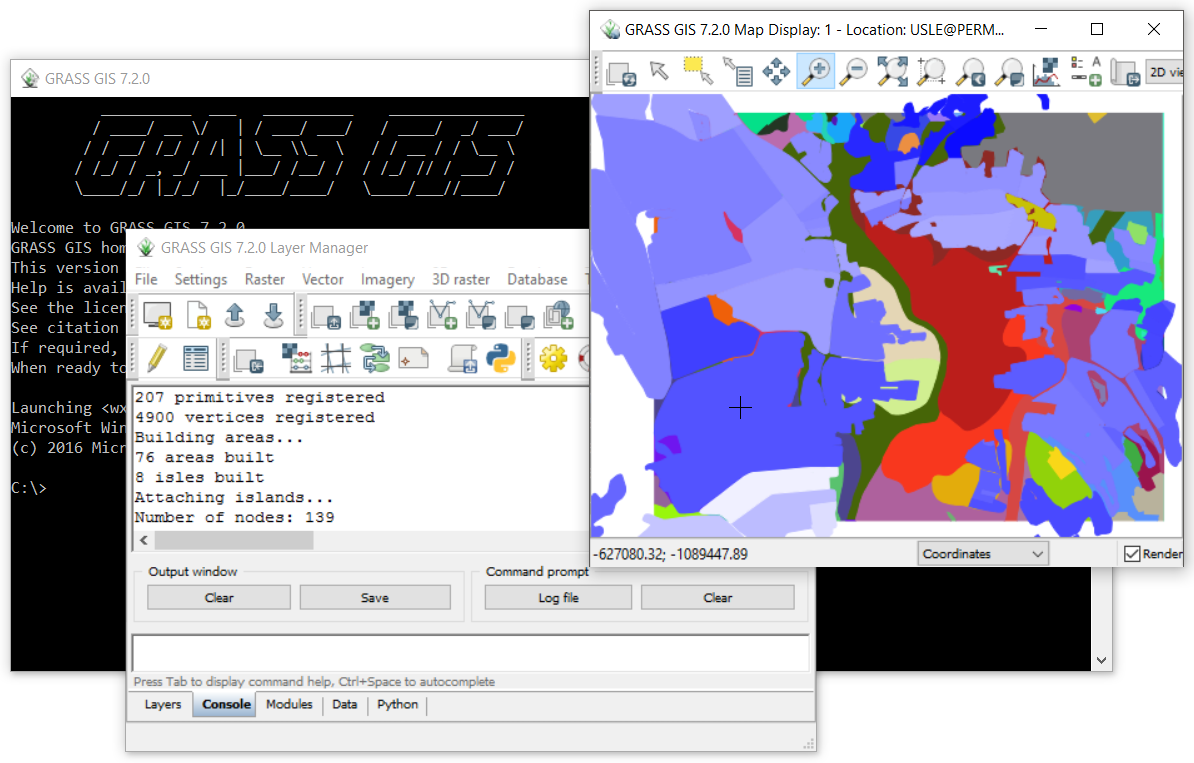
\includegraphics[scale=0.6]{./pictures/grass_screen.png}
      \caption[Náhled prostředí GRASS GIS 7.2.0]
      {Náhled prostředí GRASS GIS 7.2.0, zdroj: autor}
      \label{screen:grass}
\end{figure}
GRASS GIS (Geographic Resources Analysis Support System) je stejně
jako QGIS multiplatformním geografickým informačním systémem, který je
volně šiřitelný pod licencí GNU/GPL. Jeho vývoj započala U.S. Army
Corps of Enginneer/CERL (Construction Engineering Research Lab) už
počátkem 80. let, na jejich konci byly veškeré zdrojové kódy uvolněny
veřejnosti a v roce 1995 CERL z projektu odešel úplně. Další vývoj se
poté začal odehrávat na akademické půdě, především na Baylor
University v Texasu, USA a v Hannoveru v Německu. V roce 2008 byl
projekt zařazen do Open Source Geospatial Foundation.

GRASS pracuje s vektorovými i rastrovými daty pomocí modulů, kterých
je z obdobných důvodů jako u QGIS mnoho. Technika použití modulů je
spjata s dlouhou historií a počátky vývoje softwaru, kdy bylo potřeba
s výkonem procesoru i využitím operační paměti šetřit.

Dalším specifikem GRASS GIS je nutnost pracovat s daty v pevně
definované adresářové struktuře, díky čemuž je uživatel nucen data
systematizovat. Struktura je rozdělena na databázi, lokaci a mapset.
%%% ML: k pomlckach, tady chcete vyctove prostredi (itemize/enumerate)?
%%% RN: ano, text nebyl v dobe kontroly finalne upraven, opraveno
\begin{itemize}
	\item \textbf{Databáze} (Databanka) je běžným adresářem na disku a 
	obsahuje veškerá data, ke kterým GRASS přistupuje.
	\item \textbf{Lokace} (Projekt) je adresář umístěný v databance, 
	pro který je definován souřadnicový systém a jeho obsahem jsou data 
	související s daným projektem.
	\item \textbf{Mapset} tvoří soubor map z jedné lokace, jež jsou 
	určitým způsobem logicky provázány. Součástí každé lokace je mapset 
	s názvem PERMANENT, který by měl obsahovat základní datové vrstvy.
\end{itemize}
GRASS je možné ovládat, jak z příkazové řádky, tak pomocí GUI. Další
možností je přistupovat k modulům GRASS pomocí GUI QGIS, které mnoho
uživatelů shledává přívětivějším.
\newpage
\section[Python]{Python 
\includegraphics[scale=0.2]{./pictures/python.png}
\footnote{https://www.python.org/community/logos/}}
\label{python}
Celý kód byl psán ve skriptovacím programovacím jazyce Python. Jedná
se o objektově orientovaný jazyk představený v roce 1991 Guido van
Rossumem. Python je dále vyvíjen jako open source projekt, který je
zdarma distribuován na většinu platforem. Jazyk se vyznačuje
jednoduchou, ale účelnou syntaxí, reprezentovanou např. dynamickou
kontrolou datových typů nebo definicí bloků pomocí odsazování. Výhodou
Pythonu je i jeho poměrně snadné rozšíření jazykem C, který je
výkonnější a dokáže zrychlit náročnější operace.

V současné době je stále nejvyužívanější verzí Python 2.7.x, kterou
byla druhá řada ukončena a nyní se v ní jen opravují chyby. Už od roku
2008 je ve vývoji třetí řada, ta však není zpětně kompatibilní. Proto
%%% ML: co to zname pro vas kod?
%%% RN: doplneno
je potřeba software napsaný v Python 2 pro novou verzi adaptovat. Kód 
pluginu vyvíjeného v této práci byl již vytvářen s ohledem na novou 
verzi Python 3 a měl by být kompatibilní s oběma verzemi.
\cite{diveIntoPython}\cite{learningPython}

\section[PyCharm]{Pycharm 
\includegraphics[scale=0.2]
{./pictures/pycharm.png} \footnote{https://www.jetbrains.com/pycharm/}}
\label{python}
\vspace{-10pt}
\begin{figure}[H]
    \centering 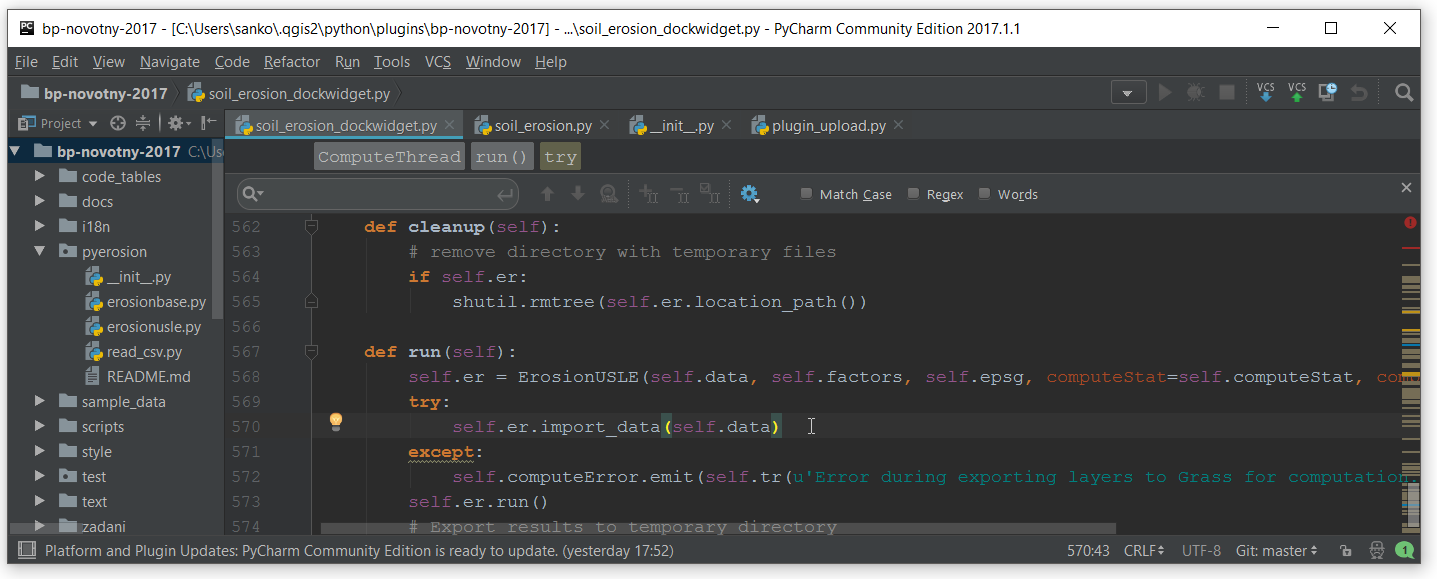
\includegraphics[scale=0.45]{./pictures/pycharm_screen.png}
      \caption[Náhled vývojového prostředí PyCharm]{Náhled vývojového 
      prostředí PyCharm, zdroj: autor}
      \label{screen:pycharm}
\end{figure}
\vspace{-10pt}
Pro vývoj zdrojového kódu bylo využito vývojové prostředí(IDE - 
Integrated Development Environment)  PyCharm, který byl vyvinut 
českou společností JetBrains. Toto prostředí bylo vytvořeno primárně 
pro Python a pro open source projekty je zdarma. Jeho výhodami jsou 
automatické doplňování textu, hledání syntaktických chyb či vytváření 
oddělených projektů. Osobně oceňuji zejména přehlednost a rychlost 
psaní kódu v tomto IDE.\cite{masteringPycharm}
\section[GitHub]{GitHub 
\includegraphics[scale=0.06]{./pictures/github.png} 
\footnote{https://github.com/}}
\label{github}
\begin{figure}[H]
    \centering 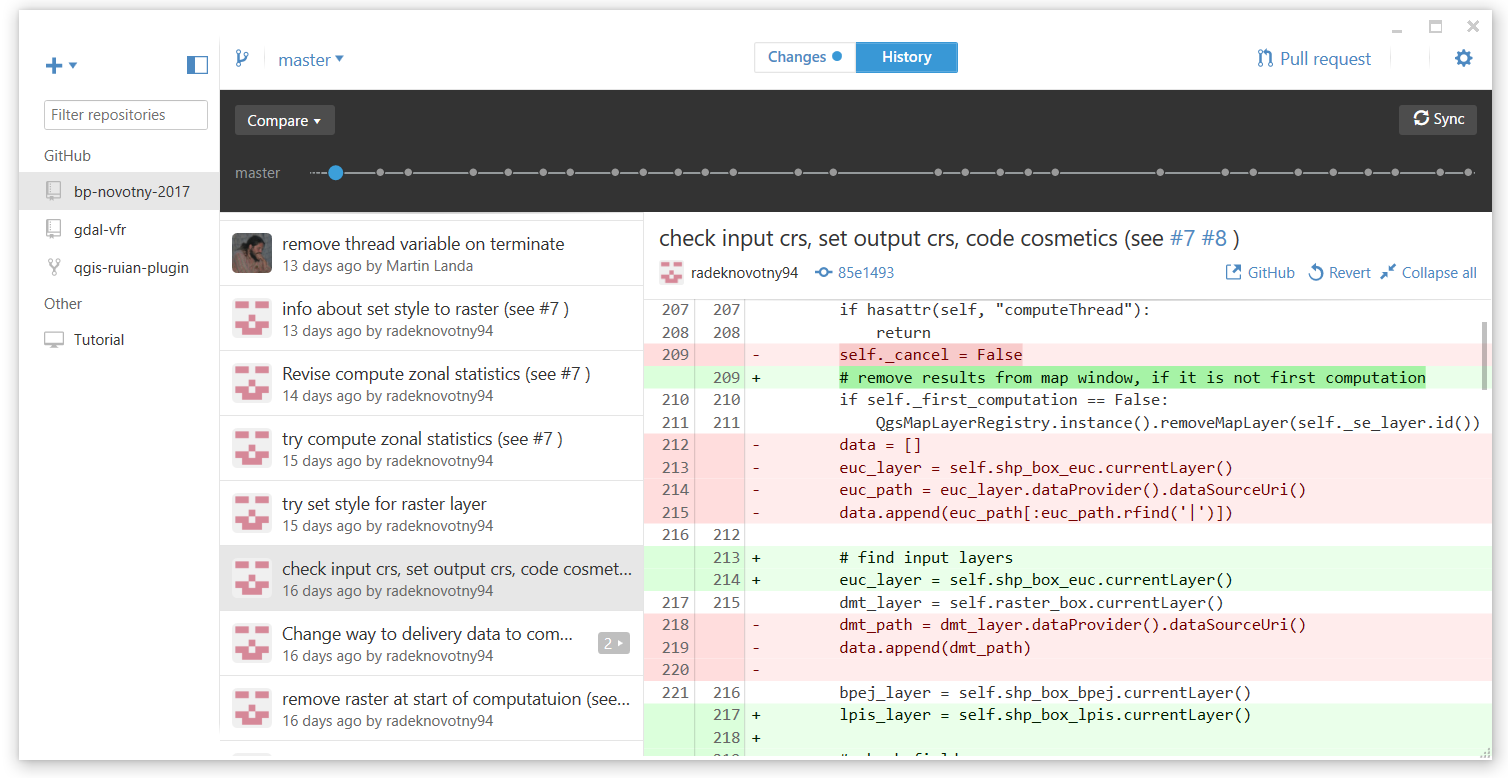
\includegraphics[scale=0.45]{./pictures/github_screen.png}
      \caption[Náhled verzovacího prostředí GitHub]
      {Náhled verzovacího prostředí GitHub, zdroj: autor}
      \label{screen:github}
\end{figure}
GitHub je webová služba podporující verzovací nástroj Git, což je distribuovaný (kolektivní) systém správy verzí. Git byl vytvořen Linusem Torvaldsem pro vývoj jádra operačního systému Linux a funguje pod licencí GNU/GPL. Na tomto základu je tedy postaven GitHub, který pro open source projekty zdarma nabízí vytvoření repositáře se zdrojovým kódem, dokumentací, historií verzování, systémem pro sledování problémů (Issue tracking), zobrazování rozdílů mezi verzemi a mnoho dalšího.\cite{introducingGithub}

\section[Qt]{Qt 
\includegraphics[scale=0.20]{./pictures/qt.png} 
\footnote{https://www.qt.io/ide/}}
\label{qt}
\begin{figure}[H]
    \centering 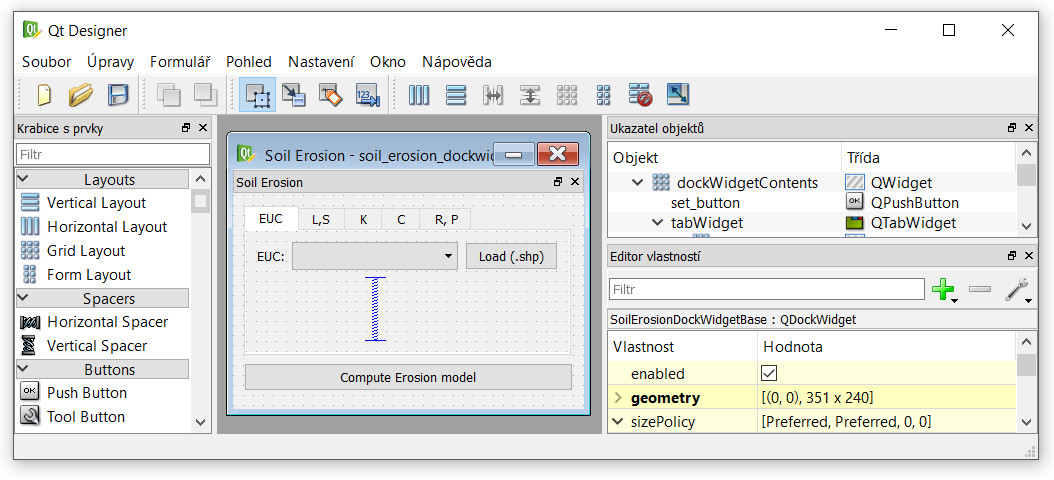
\includegraphics[scale=0.6]{./pictures/qt_screen.png}
      \caption[Náhled prostředí Qt Designer]
      {Náhled prostředí Qt Designer, zdroj: autor}
      \label{screen:qt}
\end{figure}
Qt je multiplatformní aplikační framework, který je využíván pro
tvorbu aplikací s grafickým uživatelským rozhraním (GUI). Qt toolkit
byl vytvořen v roce 1999 firmou Trolltech, v roce 2008 jej odkoupila
společnost Nokia, která je stále hlavním vývojářem toolkitu, přestože
v roce 2011 prodala licenci na komerční projekty vytvořené v Qt firmě
Digia.

Hlavními aplikacemi jsou Qt Creator, sloužící ke kompletní tvorbě
aplikací, a Qt Designer, pomocí kterého je navrhováno samotné
GUI. Výhodou je přizpůsobení výsledného GUI nativnímu vzhledu
operačního systému. Qt podporuje používání řady jazyků, od výchozího
C++ po Python, který je na Qt navázán pomocí frameworku PyQt.\cite{qt}
\cite{rapidPyQt}
